\documentclass[conference]{IEEEtran}
\IEEEoverridecommandlockouts
% The preceding line is only needed to identify funding in the first footnote. If that is unneeded, please comment it out.
\usepackage{cite}
\usepackage{amsmath,amssymb,amsfonts}
\usepackage{algorithmic}
\usepackage{graphicx}
\usepackage{textcomp}
\usepackage{xcolor}
\usepackage{ctex}
\usepackage{fontspec}
\usepackage{listings}

\def\BibTeX{{\rm B\kern-.05em{\sc i\kern-.025em b}\kern-.08em
    T\kern-.1667em\lower.7ex\hbox{E}\kern-.125emX}}
\begin{document}

\title{数字图像处理实践报告}

\author{\IEEEauthorblockN{黄润华}
\IEEEauthorblockA{\textit{中国海洋大学} \\
email@noreply.com}}

\maketitle

\begin{abstract}
本报告为数字图像处理课程中期实践报告,内容涵盖图像增强、图像去噪、边窗滤波与维纳滤波等。报告内仿真内容部分均采用Matlab编程语言实现,仿真软件环境为Matlab R2021b,设备处理器为Apple M1,运行内存为16GB。
\end{abstract}

\begin{IEEEkeywords}
    image enhancement, image denoising, side window filter, Wiener filter
\end{IEEEkeywords}

\section{实践内容}
\begin{itemize}
    \item[1.] 任意选择一个灰度图像,应用全局直方图均衡化进行图像增强;用自适应直方图均衡化方法 (AHE)进行图像增强,改变局部图像块的大小,讨论结果的不同。
    \item[2.]选择测试图像(Iena 灰度图或其它),添加高斯噪声(低,中高水平),运用下列几种方式去噪:高斯低通, 小波去噪, 双边滤波,非局部均值.
    \item[3.] 查找有关“边窗滤波”的文献和算法实现,要求:简要叙述其原理;进行实验验证(任意选择测试图像,与任务2的结果比较) 
    \item[4.] 选择测试图像(Lena 灰度图或其它),经高斯低通滤波变模糊,再加上高斯噪声后成为退化图像,应用维纳滤波复原方法对其复原,给出不同噪声水平下的复原结果 
\end{itemize}

\section{仿真结果}
\subsection{全局直方图均衡化结果}
\begin{figure}[htbp]
	\centerline{
		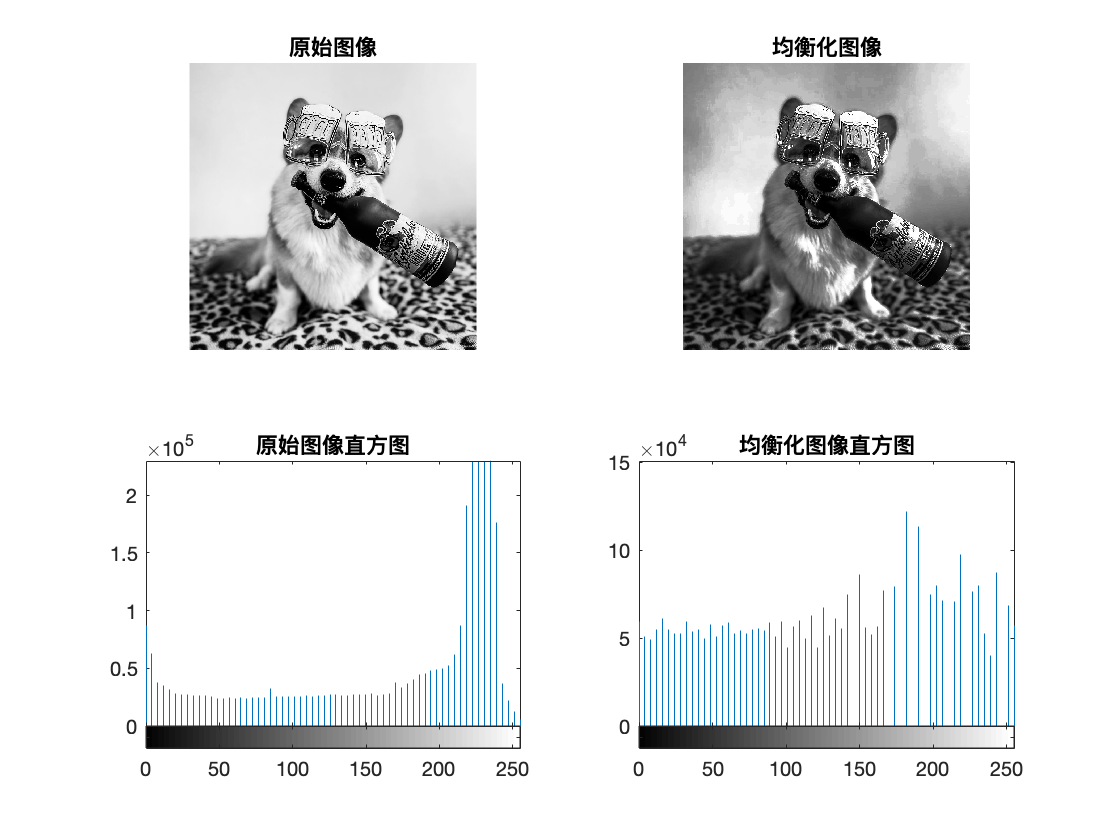
\includegraphics[width=10cm]{q1_1.png} 	
	}
	\caption{全局直方图均衡化结果}
	\label{pic1}
\end{figure}

图\ref{pic1}显示了应用全局直方图均衡化进行图像增强的最终结果。其中第一行图片分别代表原始灰度图像与直方图均衡化后的图像;第二行分别显示了直方图均衡化前后图像的直方图信息。从直方图可以直观的看出在进行直方图均衡化后,原始图像的直方图变成均匀分布的形式,同时从图像本身对比可以发现,添加直方图均衡化后的图像整体对比度效果明显增强。

\subsection{自适应直方图均衡化结果}
\begin{figure}[htbp]
	\centerline{
		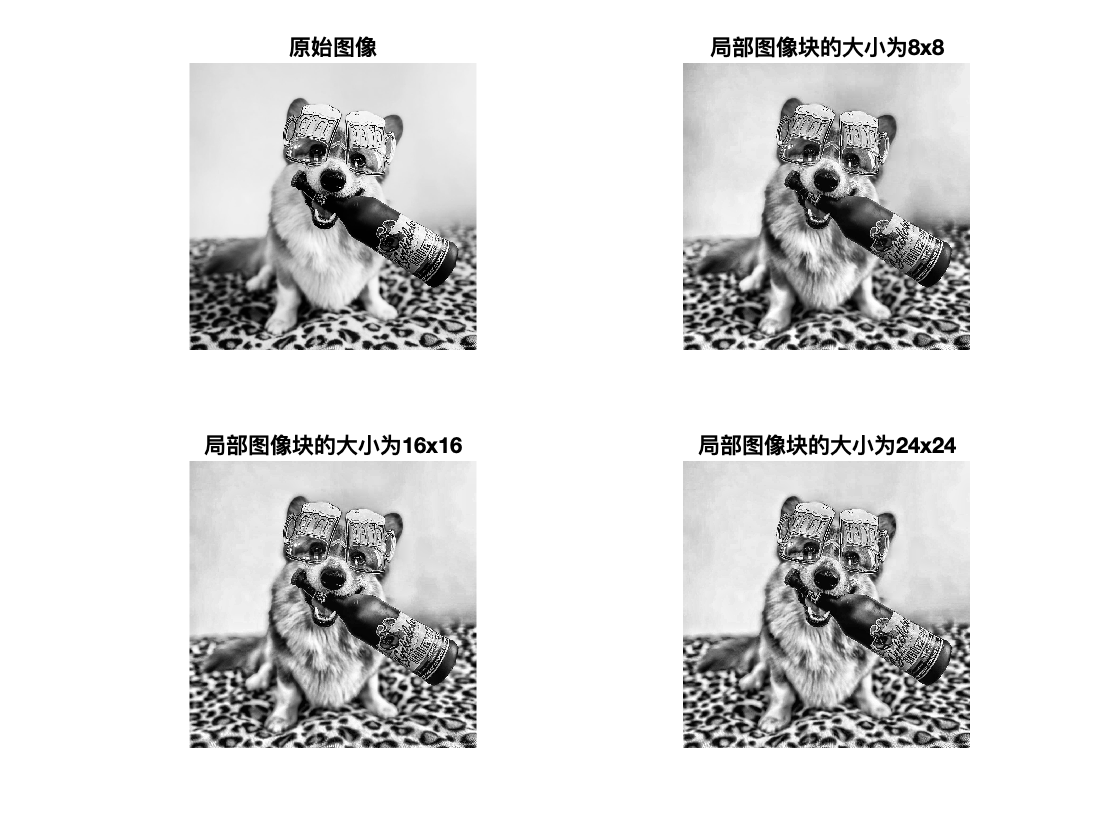
\includegraphics[width=10cm]{q1_2.png} 	
	}
	\caption{自适应直方图均衡化结果}
	\label{pic2}
\end{figure}

图\ref{pic2}显示了应用自适应直方图均衡化进行图像增强的最终结果。其中第一行图片分别代表原始灰度图像与采用局部图像块大小为$8\times 8$自适应直方图均衡化后的图像;第二行分别为采用局部图像块大小为$16\times 16$自适应直方图均衡化后的图像与采用局部图像块大小为$24\times 24$自适应直方图均衡化后的图像。

通过图像的对比可以看出使用自适应直方图均衡化方法后图像的局部对比度增强,同时图像细节更加细腻饱满。同时,随着采用的局部图像块大小的增大,图像的细节随之增多,局部对比度也呈现正相关的增长。这表明自适应直方图均衡化方法适合于改进图像的局部对比度以及获得更多的图像细节。

\subsection{高斯低通滤波去噪结果}
\begin{figure}[htbp]
	\centerline{
		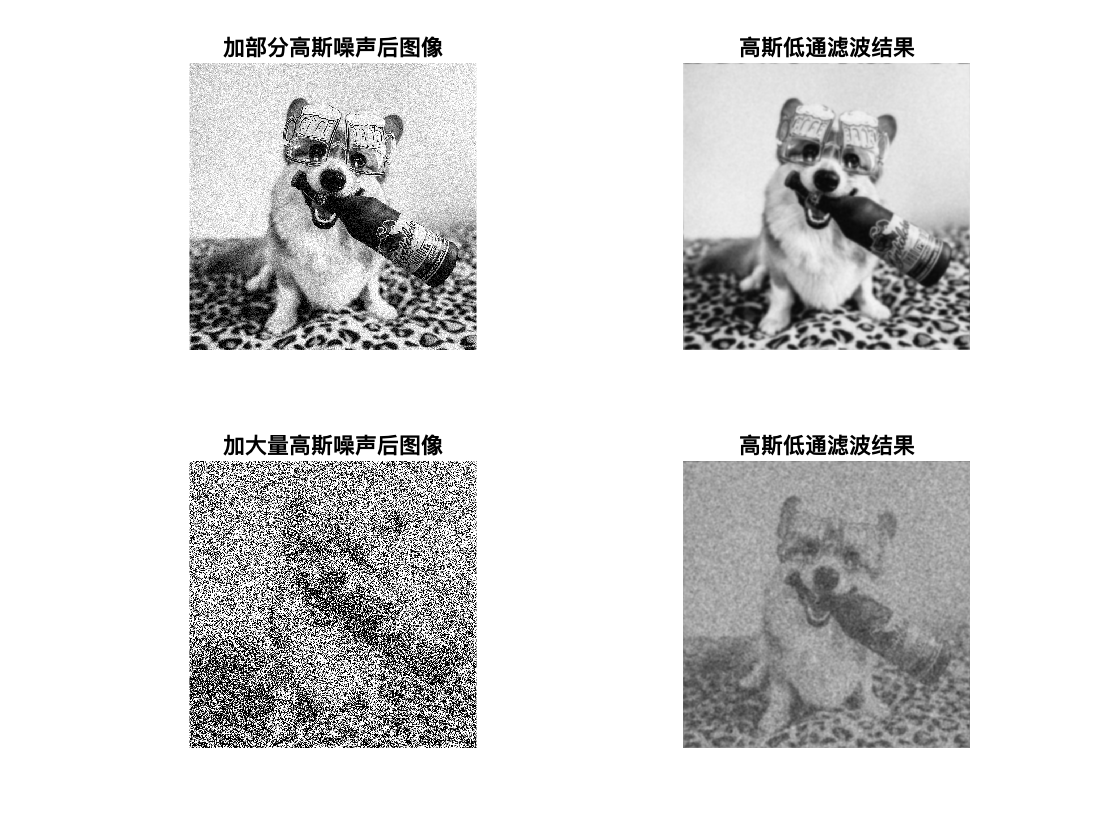
\includegraphics[width=10cm]{GL.png} 	
	}
	\caption{高斯低通滤波去噪结果}
	\label{pic3}
\end{figure}

图\ref{pic3}左边一列显示了对灰度图像添加不同水平的高斯噪声后的结果,可以明显看出,随着加入的高斯噪声的增多,图片的模糊程度逐渐增加,图片愈发难以辨认。

图\ref{pic3}右边一列显示了添加高斯噪声后的灰度图片进行高斯低通滤波的结果。通过对比第一行两张图片可以看出,经过高斯低通滤波后的图像去除了较多的噪点,保留了原始图片较多的细节,但出现了边际模糊的现象。在处理含有大量噪声的图片时,高斯低通对图像噪声的抑制较为明显,同时滤波后的图像具备原始图像的大致轮廓。

\subsection{小波去噪结果}
\begin{figure}[htbp]
	\centerline{
		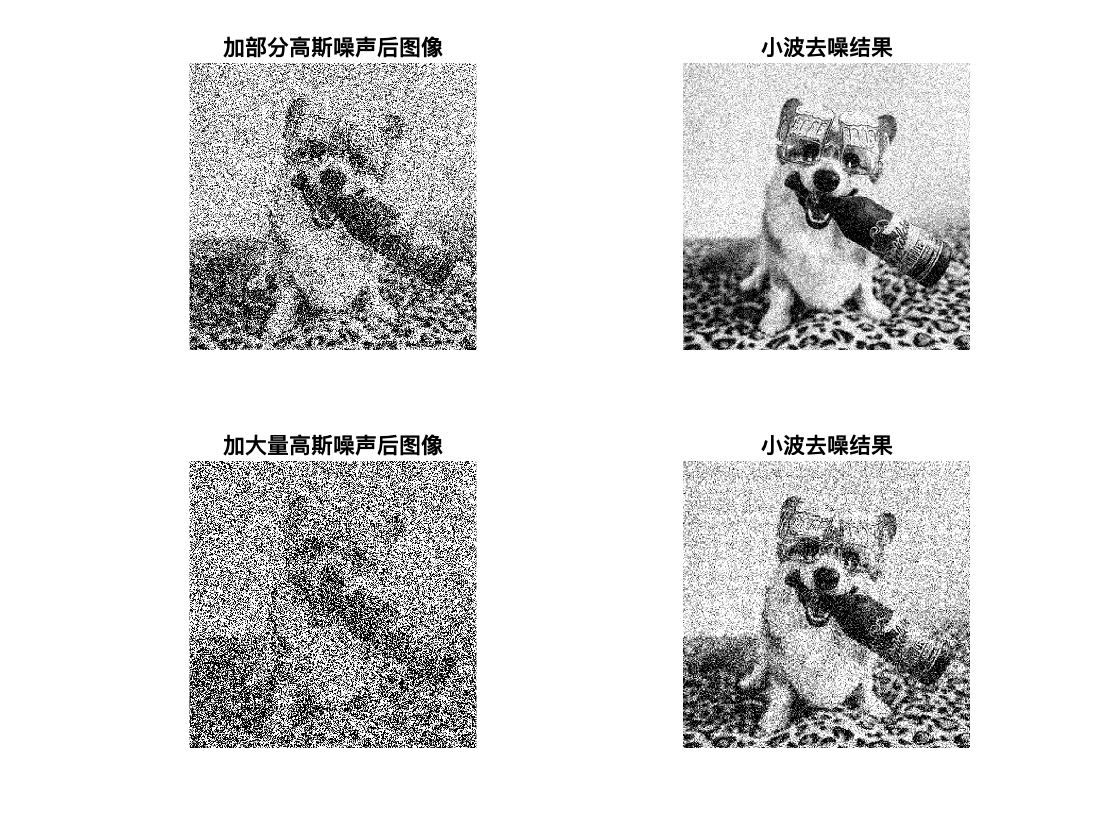
\includegraphics[width=10cm]{LW滤波结果.png} 	
	}
	\caption{小波去噪结果}
	\label{pic4}
\end{figure}

图\ref{pic4}左边一列显示了对灰度图像添加不同水平的高斯噪声后的结果,可以明显看出,随着加入的高斯噪声的增多,图片的模糊程度逐渐增加,图片愈发难以辨认。

图\ref{pic4}右边一列显示了添加高斯噪声后的灰度图片进行小波去噪的结果。通过对比第一行两张图片可以看出,经过小波去噪后的图像去除了较多的噪点,保留了原始图片较多的细节。在处理含有大量噪声的图片时,小波去噪对图像噪声的抑制较为明显,同时滤波后的图像具备原始图像的大致轮廓。对比图\ref{pic4}与图\ref{pic3}的第二行可以发现,相比于高斯低通滤波的方法,小波去噪对图像噪声的抑制较为明显。

\subsection{双边滤波结果}
\begin{figure}[htbp]
	\centerline{
		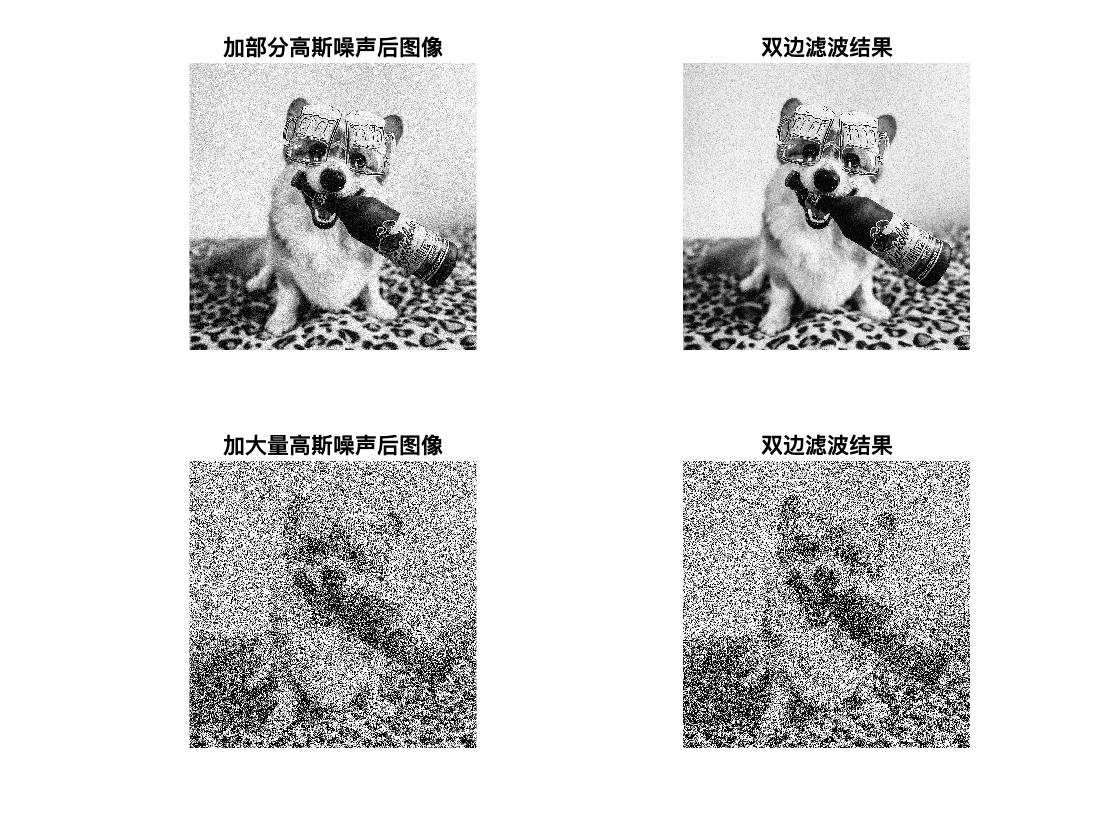
\includegraphics[width=10cm]{DF滤波结果.png} 	
	}
	\caption{双边滤波结果}
	\label{pic5}
\end{figure}

图\ref{pic5}左边一列显示了对灰度图像添加不同水平的高斯噪声后的结果,可以明显看出,随着加入的高斯噪声的增多,图片的模糊程度逐渐增加,图片愈发难以辨认。

图\ref{pic5}右边一列显示了添加高斯噪声后的灰度图片进行双边滤波的结果。通过对比第一行两张图片可以看出,经过双边滤波后的图像去除了较多的噪点,保留了原始图片较多的细节。同高斯低通滤波相比,双边滤波后的图像没有出现图片边缘模糊化的现象。然而在处理含有大量噪声的图片时,双边滤波对图像噪声的抑制较差。

\subsection{非局部均值滤波结果}
\begin{figure}[htbp]
	\centerline{
		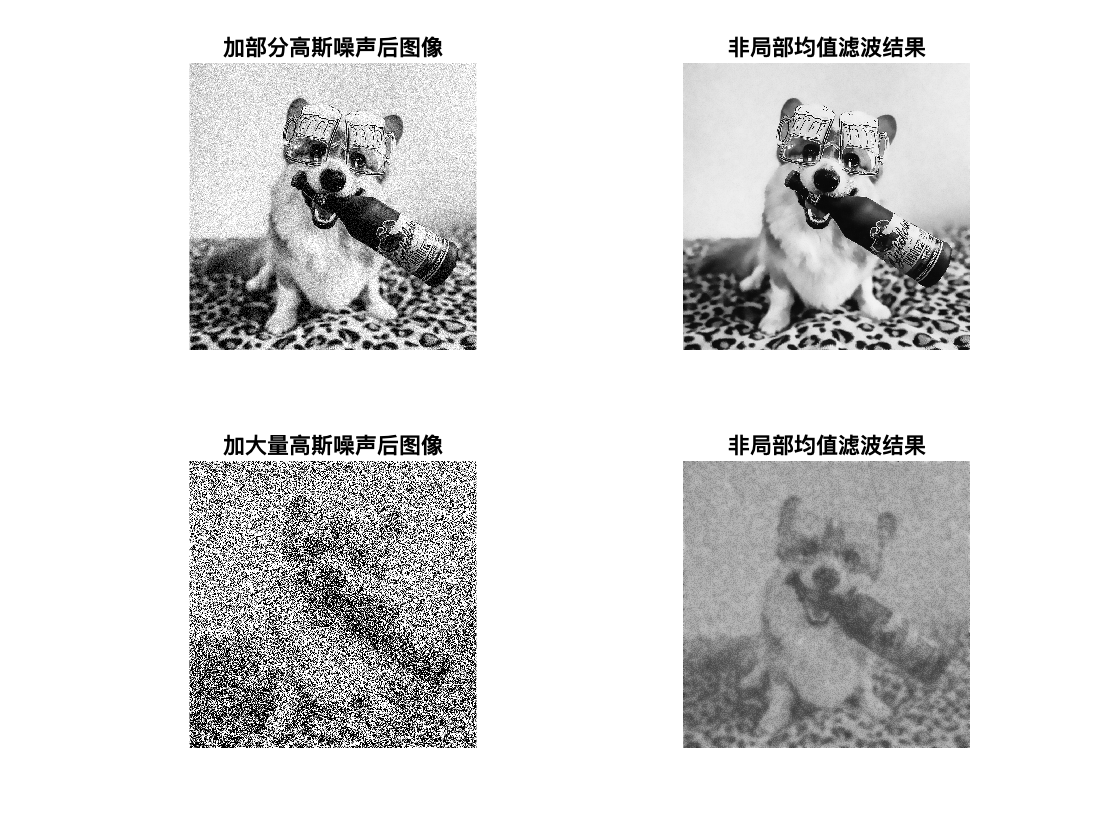
\includegraphics[width=10cm]{NLM滤波结果.png} 	
	}
	\caption{非局部均值滤波结果}
	\label{pic6}
\end{figure}

图\ref{pic6}左边一列显示了对灰度图像添加不同水平的高斯噪声后的结果,可以明显看出,随着加入的高斯噪声的增多,图片的模糊程度逐渐增加,图片愈发难以辨认。

图\ref{pic6}右边一列显示了添加高斯噪声后的灰度图片进行非局部均值滤波的结果。通过对比第一行两张图片可以看出,经过非局部均值滤波后的图像去除了较多的噪点,保留了原始图片较多的细节。同高斯低通滤波相比,非局部均值滤波后的图像没有出现图片边缘模糊化的现象。在处理含有大量噪声的图片时,非局部均值滤波后的图像可以大致反映原始图像的轮廓。

\section{边窗滤波}
\subsection{边窗滤波原理}
边窗滤波本质上为保边滤波策略,核心思想在于将每个滤波像素点都当成是潜在的边缘点,对于每个待滤波的像素点,生成几种不同的滤波子窗口,将生成的滤波子窗口的边缘或者角点位置同待滤波的像素点对齐,进行滤波得到结果,根据子窗口的滤波之后的最佳重构结果作为最终的滤波结果。

\subsection{边窗滤波仿真结果}

\end{document}
